\documentclass[runningheads,a4paper]{llncs}
\usepackage{amssymb}
\usepackage{amsmath}
\usepackage{subfig}
\setcounter{tocdepth}{3}
\usepackage{graphicx}
%\usepackage{titlesec}
\usepackage[hidelinks]{hyperref}
\usepackage{listings}

\usepackage[english, spanish]{babel}
%\usepackage[utf8]{inputenc}
\usepackage{url}
\urldef{\mailsa}\path|https://github.com/hbm99/bias-project-ML.git|    
\newcommand{\keywords}[1]{\par\addvspace\baselineskip
	\noindent\keywordname\enspace\ignorespaces#1}


\begin{document}
	
	\title{Proyecto de \\Aprendizaje de M\'aquinas}
	
	%titulo del problema
	%\titlerunning{Estado del Arte}
	
	
	\author{ Daniela Rodr\'iguez Cepero\\ Elena Rodr\'iguez Horta\\ Hasel Mart\'i Blanco\\ Karel Camilo Manresa Le\'on\\ Karlos Alejandro Alfonso Rodr\'iguez\\ L\'azaro Alejandro Castro }
	
	
	\institute{Universidad de La Habana,\\
		San L\'azaro y L. Plaza de la Revoluci\'on, La Habana, Cuba\\
		\mailsa\\
		\url{http://www.uh.cu}}
	
	
	\maketitle
	
	%\mainmatter 
	\newpage
	\tableofcontents
	
	
\newpage	
\section{Introducci\'on}
Hace unos a\~nos, al hablar de modelos de inteligencia artificial (IA), pr\'acticamente se asum\'ia que nos reg\'iamos a unos contextos muy concretos y exclusivos: grandes empresas tecnol\'ogicas, centros de investigaci\'on en la materia y entornos similares. Esta situaci\'on ha cambiado dr\'asticamente al d\'ia de hoy.\\

En la actualidad esos modelos de IA est\'an en nuestros tel\'efonos m\'oviles, la smart TV de nuestro sal\'on, hablando exclusivamente de dispositivos f\'isicos. Tambi\'en est\'an integrados en nuestro software de correo, en las redes sociales y muchos de los servicios telem\'aticos que usamos a diario. Fuera del \'ambito personal, si no nos restringimos y abrimos el abanico a entornos empresariales e institucionales, los procesos en los que se recurre a 
modelos generados por algoritmos de aprendizaje autom\'atico son incontables.\\

El creciente impacto de los modelos de aprendizaje autom\'atico en la sociedad, as\'i
como la variedad de campos en los que son aplicados, ha llamado la atenci\'on de la comunidad hacia las consecuencias que estos algoritmos pueden traer para las personas
y la sociedad de forma general. En particular, preocupan los efectos que puedan tener
en \'areas como las de la educaci\'on y formaci\'on, el empleo, los servicios, la legalidad
y los sistemas judiciales. Se ha vuelto necesario que los sistemas de inteligencia
artificial sean desarrollados con responsabilidad, teniendo en cuenta aspectos como la
imparcialidad, seguridad y privacidad, comprensibilidad honestidad y ecuanimidad resultan esenciales.\cite{Toma}.\\

Algunos gobiernos usan los modelos de aprendizaje autom\'atico en la
predicci\'on de brotes virales y focos de cr\'imenes. Los sesgos existentes en estos modelos tienen repercusiones trascendentales, lo cual es preocupante por el hecho de que pueden reforzarse o derivar en resultados inesperados\cite{K}.\\

El proceso de contrataci\'on se ha convertido en un proceso automatizado en muchos casos, desde la selecci\'on de curr\'iculums hasta la elecci\'on de los candidatos.
Como consecuencia de la participaci\'on cada vez mayor de sistemas automatizados
y de aprendizaje autom\'atico en esta tarea de gran repercusi\'on para las personas, es
necesario controlar cu\'ando una decisi\'on es injusta \cite{Candice}.\\

De manera general, en la comunidad existen posiciones diferentes acerca del uso de
los algoritmos de aprendizaje autom\'atico en la toma de decisiones. Algunos plantean
que el uso de algoritmos en la toma de decisiones, en particular en la evaluaci\'on de
riesgo en escenarios judiciales, debe ser detenido, pues estos modelos son fuentes de
incertidumbres y alteraciones \cite{Pascal}.\\

 Considerando las definiciones de equidad presentes
en la literatura, existen numerosos algoritmos de clasificaci\'on que tienen un buen
desempe\~no. Sin embargo, debido a que estos se enfocan en el tiempo presente y dado
que incorporan el sesgo humano, existe el riesgo y la propensi\'on a repetir y aumentar
dichos sesgos \cite{Paaben}.\\

Teniendo en cuenta los riesgos que supone la utilizaci\'on de los modelos de aprendizaje
autom\'atico en la toma de decisiones, es necesario enfrentar los sesgos y prejuicios
que contienen para que no se mantengan y extiendan. Es importante implementar
conceptos \'eticos fundamentales en la inteligencia artificial \cite{Claudio} y construir sistemas que
se comprometan con los valores sociales \cite{Julia}. Es decir, determinar cu\'an dañino
puede ser un sesgo y, por tanto, cu\'ales no pueden ser permitidos en los algoritmos. Es una tarea dif\'icil pero sumamente necesaria por lo que requiere la atenci\'on de todos.

\newpage
\section{Sesgo}

Durante los \'ultimos a\~nos, con el creciente uso de este tipo de tecnolog\'ias, se han ido descubriendo m\'ultiples sesgos de Machine Learning que nos deber\'ian dar qu\'e pensar. Si bien el aprendizaje autom\'atico ofrece una fuente de informaci\'on muy valiosa y nos dota de herramientas de gran utilidad para comprender el mundo que nos rodea, los sesgos descubiertos podr\'ian resultar contraproducentes para el inter\'es general o beneficiar a algunos en detrimento de otros.\\

El sesgo en aprendizaje autom\'atico, tambi\'en conocido como sesgo de modelo, es la diferencia entre el valor medio predicho por el modelo y el valor medio real, aparece cuando un modelo produce resultados err\'oneos de forma sistem\'atica. La aparici\'on de estos es debida a que los modelos son desarrollados por personas. Las cuales tiene tienen preferencias que transfieren a los modelos. Tanto sean conscientes como inconscientes. Muchas veces estas pueden pasar desapercibidos hasta que los modelos se ponen en producci\'on.\\

En los procesos de toma de decisiones el t\'ermino sesgo tiene generalmente connotaciones negativas. No es deseable que un proceso autom\'atico lo tenga de ning\'un tipo. La palabra sesgo procede de sesgar, un verbo que hace referencia a torcer o atravesar algo hacia uno de sus lados. Por lo que una decisi\'on sesgada, que se tuerce en alg\'un sentido, no es deseable. Los modelos de aprendizaje autom\'atico (“machine learnig”) no est\'an exentos de este problema, ya que son desarrollados por personas. As\'i que es importante conocer qu\'e es el sesgo en aprendizaje autom\'atico y c\'omo se puede minimizar su aparici\'on.\\

Debido a todo esto se ha dirigido el estudio de muchos investigadores hacia la detecci\'on de sesgos en sistemas existentes por ejemplo existe un estudio que analiza y eval\'ua los sesgos existentes en los algoritmos y conjuntos de datos de an\'alisis facial automatizados 
(tales como IARPA Janus Benchmark-A(IJB-A) y Adience \cite{Joy}). En \'el se plantea la relevancia que puede tener en el an\'alisis de los datos los subgrupos que se consideran, que pueden constituir la diferencia entre encontrar sesgos o no.\\

Varios sistemas de NLP usan los vectores (embeddings) de palabras, que son una
forma de representarlas y capturar sus asociaciones y sem\'antica. Estos vectores son
construidos a partir de los contextos en que aparecen las palabras en los textos.
Varios estudios se han enfocado en el reconocimiento de sesgos en estos vectores. Uno
de ellos reconoce sesgos presentes en vectores generados por modelos como GloVe \cite{Jef},
y Word2Vec \cite{Tomas}, entrenado con los art\'iculos de Google News \cite{Tolga}.\\

Los prejuicios y sesgos existentes en la sociedad han sido detectados tambi\'en en
cuerpos documentales como Wikipedia. Esto se refleja en las diferencias entre las
formas en las que las mujeres y los hombres son descritos \cite{Claudia}. Anuncios generados
por modelos de aprendizaje autom\'atico \cite{Lat}, así como los motores de b\'usqueda en
la Web \cite{Kay} han sido detectados como fuentes de sesgos, por ejemplo, de g\'enero. Otros
ejemplos de sistemas en los que se han detectado sesgos son los chatbots, los sistemas
de reconocimiento facial y de voz
, y algunos sistemas empleados en concursos de
belleza.

s. COMPAS (Correctional Offender Management
Profiling for Alternative Sanctions) es un software usado en las cortes de Estados
Unidos para determinar la probabilidad de que una persona reincurra en un crimen.
Se encontr\'o que el software estaba sesgado hacia los afroamericanos \cite{Lauren}. Esto quiere
decir que, dados dos individuos con el mismo perfil, bastaba con que se diferenciaran
\'unicamente en que uno fuera afroamericano y el otro no para asociarle un mayor riesgo
al primero. COMPAS es usado por los jueces para decidir si liberar a un prisionero o
mantenerlo en la c\'arcel. Se ha mostrado que COMPAS no es m\'as preciso que otros
sistemas m\'as simples que tienen el mismo objetivo, ni siquiera toma decisiones m\'as
imparciales que las que pueden tomar personas con ning\'un conocimiento judicial \cite{JuliaD}


\subsection{Tipos de Sesgos}

Los investigadores han identificado tres categor\'ias principales de sesgo en la IA:\\
\begin{itemize}

\item {\bf Sesgos T\'ecnicos: } Se relaciona con el sesgo que empeora el prejuicio preexistente causado por uno de los procesos de decisi\'on internos del algoritmo. Es decir son los sesgos provenientes del algoritmo.\\

 El sesgo emergente ocurre como resultado del uso y la interacci\'on con usuarios reales. Este sesgo surge 
como resultado del cambio en la poblaci\'on, los valores culturales o el conocimiento social, generalmente alg\'un tiempo 
despu\'es de la finalizaci\'on del diseño. Este tipo de sesgo es m\'as probable que se observe en las interfaces de usuario, 
ya que las interfaces tienden a reflejar las capacidades, caracter\'isticas y h\'abitos de los posibles usuarios por diseño . 
Este tipo de sesgo se puede dividir en m\'as subtipos, como se analiza en detalle en la Referencia.\cite{Bat}\\

Los sesgos populares se ponen de manifiesto por ejemplo cuando los art\'iculos que son m\'as populares tienden a estar m\'as expuestos.
 Sin embargo, las m\'etricas de popularidad est\'an sujetas a manipulaci\'on, por ejemplo, por rese\~nas falsas o bots sociales . Por ejemplo,
  este tipo de sesgo se puede ver en los motores de b\'usqueda  o en los sistemas de recomendaci\'on 
donde los objetos populares se presentar\'ian más al p\'ublico. Pero esta presentaci\'on puede no ser el resultado de una buena 
calidad; en cambio, puede deberse a otros factores sesgados.\\\cite{Aza}

\item {\bf Preexistentes:} Se refiere al sesgo ya presente en los datos utilizados para entrenar el modelo de IA.\\

El sesgo hist\'orico es el sesgo y los problemas sociot\'ecnicos ya existentes en el mundo y puede filtrarse 
desde el proceso de generaci\'on de datos incluso con un muestreo y una selecci\'on de caracter\'isticas perfectos \cite{Ha}. Un 
ejemplo de este tipo de sesgo se puede encontrar en un resultado de b\'usqueda de im\'agenes de 2018 donde la b\'usqueda 
de directoras ejecutivas result\'o en \'ultima instancia en menos im\'agenes de directoras ejecutivas debido al hecho de que 
solo el 5 \%  de las directoras ejecutivas de Fortune 500 eran mujeres, lo que provocar\'ia que los resultados de la b\'usqueda 
estar sesgado hacia los directores ejecutivos masculinos \cite{Ha}. Estos resultados de b\'usqueda, por supuesto, reflejaban la 
realidad, pero vale la pena considerar si los algoritmos de b\'usqueda deben o no reflejar esta realidad.\\

El sesgo social ocurre cuando las acciones de otros afectan nuestro juicio \cite{Ricardo}. Un ejemplo de este tipo de sesgo 
puede ser un caso en el que queremos calificar o revisar un \'item con una puntuaci\'on baja, pero al estar influenciados por 
otras calificaciones altas, cambiamos nuestra puntuaci\'on pensando que tal vez estamos siendo demasiado duros.\\
 
\item {\bf Sesgo Emergente:} Se produce debido a la interacci\'on con uno o m\'as usuarios.\\

El sesgo de comportamiento surge del diferente comportamiento de los usuarios entre plataformas, 
contextos o diferentes conjuntos de datos \cite{Alex}. Un ejemplo de este tipo de sesgo se puede observar en la Referencia 
[104], donde los autores muestran c\'mo las diferencias en las representaciones de emoji entre plataformas pueden resultar en
 diferentes reacciones y comportamientos de las personas y, a veces, incluso conducen a errores en la comunicaci\'on.\\
 
 El sesgo de representaci\'on surge de c\'mo tomamos muestras de una poblaci\'on durante 
el proceso de recopilaci\'on de datos \cite{Ha}. Las muestras no representativas carecen de la diversidad de la poblaci\'on, 
con subgrupos faltantes y otras anomal\'ias. La falta de diversidad geogr\'afica en conjuntos de datos como ImageNet da
 como resultado un sesgo demostrable hacia las culturas occidentales.

\end{itemize}

\subsection{M\'etricas y equidad}

 Las m\'etricas para estimar la quidad de los modelos pueden agruparse seg\'un si son m\'etricas para medir sesgos en grupos o en
individuos.\\

La mayor\'ia de medidas de equidad dependen de diferentes m\'etricas, de modo que comenzaremos por definirlas. Cuando trabajamos con un clasificador binario, tanto la clase predicha por el algoritmo como la real pueden tomar dos valores: positivo y negativo. Empecemos ahora explicando las posibles relaciones entre el resultado predicho y el real: 
\begin{itemize}
\item {\bf Verdadero positivo (TP):} Cuando el resultado predicho y el real pertenecen a la clase positiva.\\
\item {\bf Verdadero negativo (TN):} Cuando el resultado predicho y el real pertenecen a la clase negativa.\\
\item {\bf Falso positivo (FP): }Cuando el resultado predicho es positivo pero el real pertenece a la clase negativa.\\
\item {\bf Falso negativo (FN): }Cuando el resultado predicho es negativo pero el real pertenece a la clase positiva.\\
\end{itemize}
    
Estas relaciones pueden ser representadas f\'acilmente con una matriz de confusi\'on, una tabla que describe la precisi\'on de un modelo de clasificaci\'on. En esta matriz, las columnas y las filas representan instancias de las clases predichas y reales, respectivamente.\\

Utilizando estas relaciones, podemos definir m\'ultiples m\'etricas que podemos usar despu\'es para medir la equidad de un algoritmo: \\

\begin{itemize}
   \item {\bf Valor predicho positivo (PPV):} la fracci\'on de casos positivos que han sido predichos correctamente de entre todas las predicciones positivas. Con frecuencia, se denomina como precisi\'on, y representa la probabilidad de que una predicci\'on positiva sea correcta. Viene dada por la siguiente f\'ormula:

${\displaystyle PPV=P(actual=+|prediction=+)={\frac {TP}{TP+FP}}}$\\

   \item {\bf Tasa de descubrimiento de falsos (FDR):} la fracci\'on de predicciones positivas que eran en realidad negativas de entre todas las predicciones positivas. Representa la probabilidad de que una predicci\'on positiva sea err\'onea, y viene dada por la siguiente f\'ormula:

${\displaystyle FDR=P(actual=-|prediction=+)={\frac {FP}{TP+FP}}}$\\

   \item {\bf Valor predicho negativo (NPV):} la fracci\'on de casos negativos que han sido predichos correctamente de entre todas las predicciones negativas. Representa la probabilidad de que una predicci\'on negativa sea correcta, y viene dada por la siguiente f\'ormula:

${\displaystyle NPV=P(actual=-|prediction=-)={\frac {TN}{TN+FN}}}$\\

    \item {\bf Tasa de omisión de falsos (FOR):} la fracci\'on de predicciones negativas que eran en realidad positivas de entre todas las predicciones negativas. Representa la probabilidad de que una predicci\'on negativa sea err\'onea, y viene dada por la siguiente f\'ormula:

${\displaystyle FOR=P(actual=+|prediction=-)={\frac {FN}{TN+FN}}}$\\

    \item {\bf Tasa de verdaderos positivos (TPR):} la fracci\'on de casos positivos que han sido predichos correctamente de entre todos los casos positivos. Con frecuencia, se denomina como exhaustividad, y representa la probabilidad de que los sujetos positivos sean clasificados correctamente como tales. Viene dada por la f\'ormula:

${\displaystyle TPR=P(prediction=+|actual=+)={\frac {TP}{TP+FN}}}$\\

   \item {\bf Tasa de falsos negativos (FNR):} la fracci\'on de casos positivos que han sido predichos de forma err\'onea como negativos de entre todos los casos positivos. Representa la probabilidad de que los sujetos positivos sean clasificados err\'oneamente como negativos, y viene dada por la f\'ormula:

${\displaystyle FNR=P(prediction=-|actual=+)={\frac {FN}{TP+FN}}}$\\

   \item {\bf Tasa de verdaderos negativos (TNR):} la fracci\'on de casos negativos que han sido predichos correctamente de entre todos los casos negativos. Representa la probabilidad de que los sujetos negativos sean clasificados correctamente como tales, y viene dada por la f\'ormula:

${\displaystyle TNR=P(prediction=-|actual=-)={\frac {TN}{TN+FP}}}$\\

    \item {\bf Tasa de falsos positivos (FPR):} la fracci\'on de casos negativos que han sido predichos de forma err\'onea como positivos de entre todos los casos negativos. Representa la probabilidad de que los sujetos negativos sean clasificados err\'oneamente como positivos, y viene dada por la f\'ormula:

${\displaystyle FPR=P(prediction=+|actual=-)={\frac {FP}{TN+FP}}}$\\

\end{itemize}

Entre las m\'etricas de grupo m\'as usadas se encuentran:
\begin{itemize}

\item {\bf Statistical o Demographic Parity} \cite{Sa} Un algoritmo predictor Y
cumple con Demographic Parity con respecto a un atributo A con valores en el conjunto
{0,1} si se cumple: $P(Y|A = 0) = P(Y|A = 1)$. Esto implica que el valor del
atributo protegido no influye en el resultado del algoritmo Y.\\

\item {\bf Equal Opportunity } \cite{Sa} \cite{Mo} Dado un predictor binario Y
con respecto a un atributo A y salida Y , esta m\'etrica se cumple cuando la probabilidad de que una
persona de la clase 1 sea correctamente asignada sea la misma para los grupos
definidos por A = 1 y A = 0, es decir, $P(Y = 1|A = 1,Y = 1) = P(Y = 1|A =0,Y = 1)$.\\

\item {\bf Equalized Odds }\cite{Mo} Un predictor Y
satisface esta m\'etrica con respecto a un
atributo protegido A, si A y el predictor son independientes dado Y , es decir,
si $P(Y = 1|A = 1,Y = y) = P(Y = 1|A = 0,Y = y)$, y $\in {0,1}$. Implica que
los grupos protegidos y los que no lo son deben tener razones iguales de falsos
positivos y verdaderos positivos.\\

\end{itemize}

Otras m\'etricas para analizar y detectar sesgos, dirigidas a los individuos, \cite{Matt} son:
\begin{itemize}
\item {\bf Fairness Through Awareness:} Individuos similares seg\'un alguna m\'etrica definida deben obtener resultados similares.\\
\item {\bf Fairness Through Unawareness:} Un algoritmo es imparcial siempre que no utilice al atributo protegido como decisor.\\
\item {\bf Conterfactual fairness:} Una decisi\'on es imparcial hacia un individuo si es la misma en el contexto real y en un contexto hipot\'etico en el que el individuo pertenece a otro grupo.\\
\end{itemize}

En cuanto a las m\'etricas para el an\'alisis y detecci\'on de sesgos, existe la posibilidad
de que al evaluar un modelo con varias m\'etricas, una de ellas detecte sesgo mientras
que las otras no. Excepto en casos especiales restringidos, satisfacer algunas de las
m\'etricas a la misma vez resulta imposible.\\

Es importante analizar el contexto y la aplicaci\'on de cada definici\'on de equidad.
No todas las definiciones se ajustan a todos los contextos y pueden tener resultados negativos si no son las adecuadas. De igual forma, analizar el tipo de sesgo es
importante a la hora de tratar de lograr la equidad.
La modelaci\'on y medici\'n temporal es importante en la evaluaci\'on de los criterios
de equidad e introduce un nuevo rango de retos en este sentido.


\section{DataSet}
{\bf Dataset:} Se define como  {\bf una colecci\'on de datos que una computadora trata como una sola unidad} . Esto significa que un conjunto de datos contiene una gran cantidad de datos separados, pero se puede usar para entrenar un algoritmo con el objetivo de encontrar patrones predecibles dentro de todo el conjunto de datos.\\

Los datos son un componente esencial de cualquier modelo de IA y, b\'asicamente, la \'unica raz\'on del aumento en la popularidad del aprendizaje autom\'atico que presenciamos hoy.\\

Generalmente un dataset se divide en varias partes, lo cual es necesario para verificar qu\'e tan bien fue el entrenamiento del modelo. Para este prop\'osito, un conjunto de datos de prueba generalmente se separa de los datos. A continuaci\'on, un conjunto de datos de validaci\'on, aunque no es estrictamente crucial, es bastante \'util para evitar entrenar su algoritmo en el mismo tipo de datos y hacer predicciones sesgadas.\\
\begin{center}
\includegraphics[scale=0.5]{img/dataset.jpg}
\end{center}

\section{Algoritmo}
Los algoritmos de aprendizaje autom\'atico son fragmentos de c\'odigo que ayudan a los usuarios a explorar y analizar conjuntos de datos complejos y a buscar significado en ellos. Cada algoritmo es un conjunto finito de instrucciones paso a paso inequ\'ivocas que puede seguir una m\'aquina para lograr un determinado objetivo. En un modelo de aprendizaje autom\'atico, el objetivo es establecer o detectar patrones que los usuarios puedan usar para hacer predicciones o clasificar información.\\

\subsection{T\'ecnicas Algor\'itmicas}
Los algoritmos de aprendizaje autom\'atico se agrupan en t\'ecnicas de aprendizaje autom\'atico que se usan par el aprendizaje supervisado, no supervisado y por refuerzo.
\begin{itemize}

\item {\bf Aprendizaje supervisado }

En el aprendizaje supervisado, la m\'aquina se ense\~na con ejemplos. De este modo, el operador proporciona al algoritmo de aprendizaje autom\'atico un conjunto de datos conocidos que incluye las entradas y salidas deseadas, y el algoritmo debe encontrar un m\'etodo para determinar c\'omo llegar a esas entradas y salidas.\\
Mientras el operador conoce las respuestas correctas al problema, el algoritmo identifica patrones en los datos, aprende de las observaciones y hace predicciones. El algoritmo realiza predicciones y es corregido por el operador, y este proceso sigue hasta que el algoritmo alcanza un alto nivel de precisi\'on y rendimiento.\\

Esta t\'ecnica es \'util cuando sabes c\'omo ser\'a el resultado. Por ejemplo, imagina que proporcionas un conjunto de informaci\'on que incluye la poblaci\'on de una serie de ciudades por a\~no durante los \'ultimos 100 a\~nos y quieres saber cu\'al ser\'a la poblaci\'on de una ciudad espec\'ifica dentro de cuatro años. El resultado utiliza etiquetas que ya existen en el conjunto de datos: poblaci\'on, ciudad y a\~no.\\

Dentro de esta t\'ecnica algunos de los algoritmos m\'as utilizados son:
\begin{itemize}
\item Algoritmos de Clasificaci\'on.
\item Algoritmos de Regresi\'on.\\\\
\end{itemize}


\item {\bf Aprendizaje sin supervisi\'on}

Aqu\'i, el algoritmo de aprendizaje autom\'atico estudia los datos para identificar patrones. No hay una clave de respuesta o un operador humano para proporcionar instrucci\'on. En cambio, la m\'aquina determina las correlaciones y las relaciones mediante el an\'alisis de los datos disponibles.\\
En un proceso de aprendizaje no supervisado, se deja que el algoritmo de aprendizaje autom\'atico interprete grandes conjuntos de datos y dirija esos datos en consecuencia. As\'i, el algoritmo intenta organizar esos datos de alguna manera para describir su estructura. Esto podr\'ia significar la necesidad de agrupar los datos en grupos u organizarlos de manera que se vean m\'as organizados.\\
A medida que eval\'ua m\'as datos, su capacidad para tomar decisiones sobre los mismos mejora gradualmente y se vuelve m\'as refinada. Esta t\'ecnica es \'util cuando no sabes c\'omo ser\'a el resultado.

Por ejemplo, imagina que proporcionas datos de clientes y quieres crear segmentos de clientes a los que les gustan productos similares. Los datos que proporcionas no est\'an etiquetados y las etiquetas de los resultados se generan en funci\'on de las similitudes detectadas entre los puntos de datos.\\

Dentro de esta t\'ecnica algunos de los algoritmos m\'as utilizados son:
\begin{itemize}
\item Algoritmos de Clustering.
\item Algoritmos de Reducci\'on de dimensionalidad.
\end{itemize}

\newpage
\item {\bf Aprendizaje por refuerzo}

El aprendizaje por refuerzo se centra en los procesos de aprendizajes reglamentados, en los que se proporcionan algoritmos de aprendizaje autom\'aticos con un conjunto de acciones, par\'ametros y valores finales.\\
Al definir las reglas, el algoritmo de aprendizaje autom\'atico intenta explorar diferentes opciones y posibilidades, monitorizando y evaluando cada resultado para determinar cu\'al es el \'optimo.\\
En consecuencia, este sistema enseña la m\'aquina a trav\'es del proceso de ensayo y error. Aprende de experiencias pasadas y comienza a adaptar su enfoque en respuesta a la situaci\'on para lograr el mejor resultado posible. Es una buena t\'ecnica para usarla en sistemas automatizados que tienen que tomar muchas decisiones pequeñas sin la intervenci\'on humana.\\
Por ejemplo, imagina que est\'as diseñando un autom\'ovil aut\'onomo y quieres asegurarse de que respeta la ley y mantiene la seguridad de los pasajeros. A medida que el coche adquiere experiencia y un historial de refuerzo, aprende a permanecer en su carril, a respetar el l\'imite de velocidad y a frenar cuando hay peatones.

\end{itemize}

\section{Modelo}

Un modelo de aprendizaje autom\'atico es un archivo, software o aplicaci\'on de computadora que se ha entrenado para juzgar y reconocer determinados tipos de patrones. Puede entrenar un modelo con un conjunto de datos, y proporcionarle un algoritmo que puede usar para aprender de esos datso y as\'i lograr averiguar y obtener informaci\'on. Una vez entrenado el modelo, puedes usarlo para desglosar los datos que no ha visto antes y realizar predicciones sobre estos.

Todos los modelos de aprendizaje autom\'atico se clasifican en supervisados, no supervisados ​​y aprendizaje reforzado.

\begin{center}
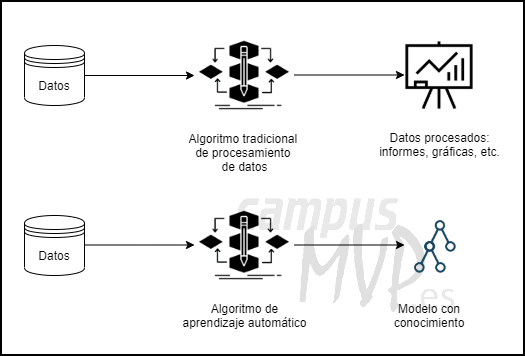
\includegraphics[scale=0.5]{img/image.png}
 \cite{link10}
\end{center}

 
 \newpage
\section{Modelo Clip de OpenAI}

CLIP (Contrastive Language-Image Pre-Training) es un modelo desarrollado por investigadores de OpenAI a principios de 2021, parece m\'as un sistema de reconocimiento de im\'agenes. Su diferencia radica en que no ha aprendido a reconocer im\'agenes a partir de ejemplos etiquetados en los conjuntos de datos seleccionados, como la mayor\'ia de los modelos existentes, sino a partir de las im\'agenes y sus descripciones publicadas en internet. CLIP aprende qu\'e hay en una imagen en funci\'on de una descripci\'on en vez de una etiqueta de una palabra como $gato$.\\

CLIP fue entrenado con la orden de predecir cu\'al de las 32.768 descripciones de una selecci\'on aleatoria era la correcta para una imagen determinada. Para lograrlo, CLIP aprendi\'o a vincular una amplia variedad de objetos con sus nombres y las palabras que los describen. Esto le permite identificar objetos en im\'agenes que no pertenecen a su conjunto de entrenamiento.\\

CLIP entrena previamente un codificador de im\'agenes y un codificador de texto para predecir qu\'e im\'agenes se emparejaron con qu\'e textos en nuestro conjunto de datos. Luego usamos este comportamiento para convertir CLIP en un clasificador de tiro cero ($zero-shot$). Convertimos todas las clases de un conjunto de datos en leyendas como {\bf una foto de un perro} y predecimos la clase de la leyenda que CLIP estima que se empareja mejor con una imagen dada.\\\\

\begin{center}
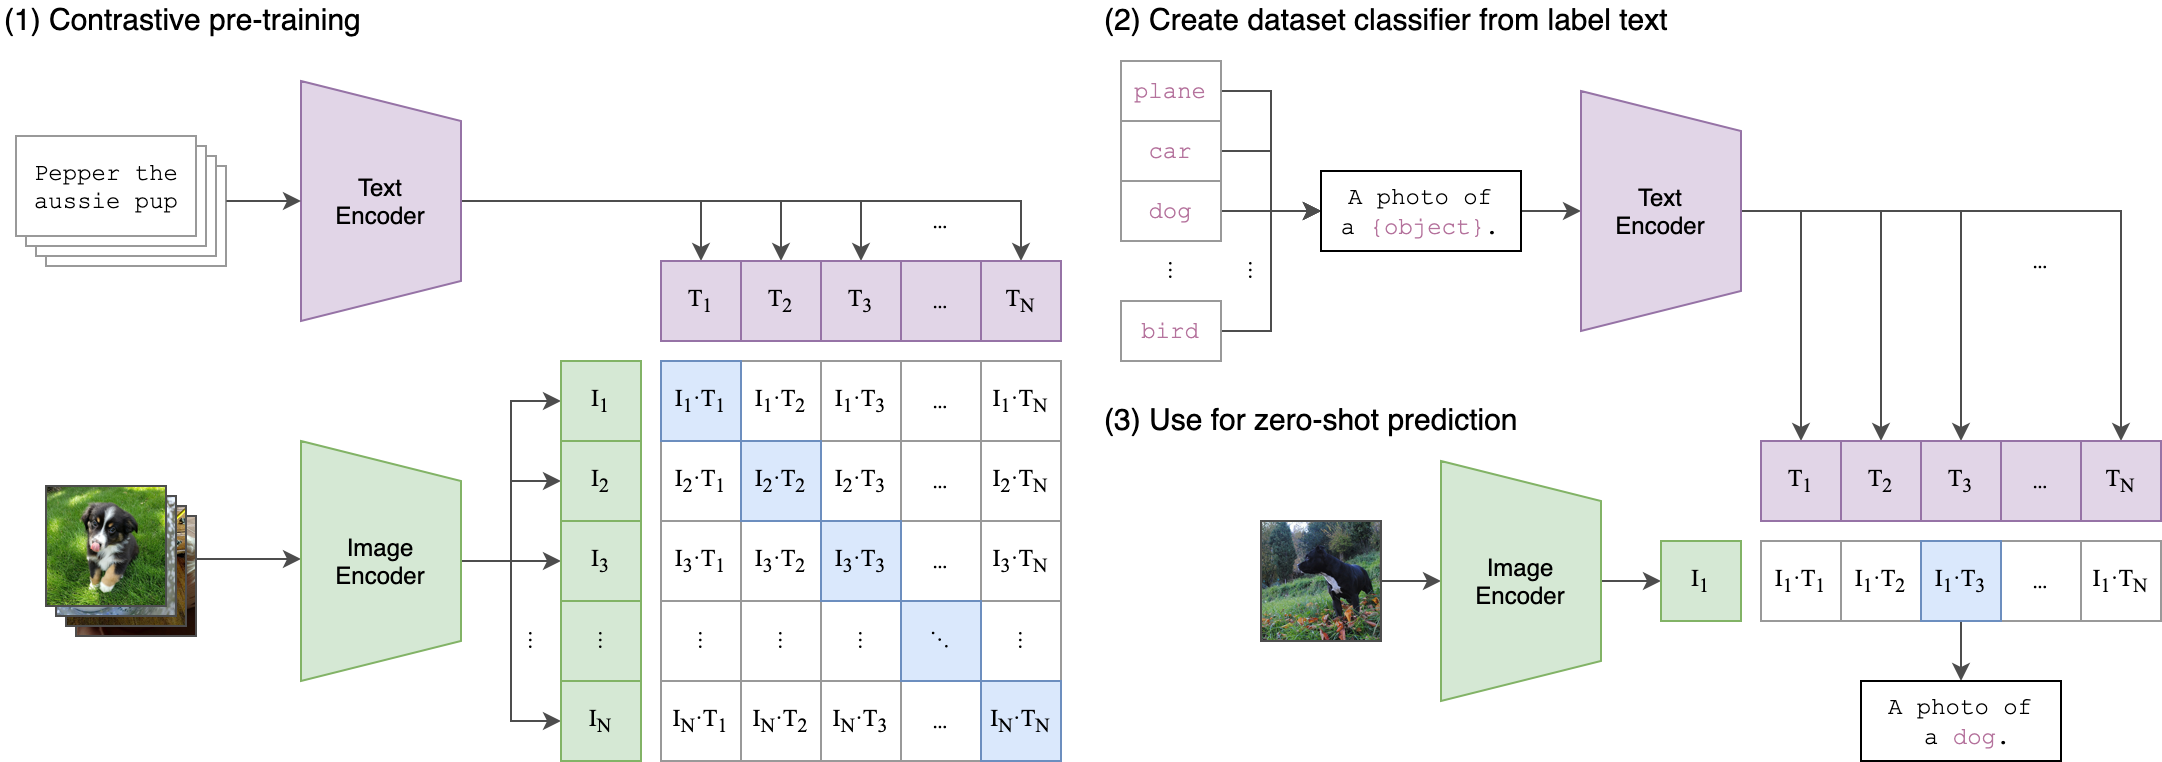
\includegraphics[scale=0.15]{img/CLIP.png}\\
 \cite{Clip}
\end{center}

La mayor\'ia de los sistemas de reconocimiento de im\'agenes se entrenan para identificar ciertos tipos de objetos, como rostros en los v\'ideos de vigilancia o edificios en las im\'agenes de sat\'elite. Al igual que GPT-3, CLIP puede generalizar entre tareas sin necesidad de entrenamiento adicional. Tambi\'en es menos propenso que otros modelos de reconocimiento de im\'agenes de \'ultima generaci\'on a dejarse enga\~nar por algunos ejemplos contradictorios, alterados sutilmente de distintas formas que suelen confundir los algoritmos, aunque las personas no noten la diferencia.\\


\newpage
% \cite[pag]{clave}
\addcontentsline{toc}{section}{Referencias}
\begin{thebibliography}{99}

\bibitem{link1} https://bytespider.eu/3-tipos-de-sesgo-en-los-modelos-de-ia-y-como-podemos-abordarlos/

\bibitem{link2} https://empresas.blogthinkbig.com/que-es-machine-bias-los-sesgos-en/

\bibitem{link3} https://www.analyticslane.com/2019/04/24/que-es-el-sesgo-en-aprendizaje-automatico/

\bibitem{link4} https://labelyourdata.com/articles/what-is-dataset-in-machine-learning

\bibitem{link5} https://keepler.io/es/2021/03/la-dicotomia-sesgo-varianza-en-modelos-de-machine-learning/

\bibitem{link6} https://azure.microsoft.com/es-es/resources/cloud-computing-dictionary/what-are-machine-learning-algorithms

\bibitem{link7} https://www.apd.es/algoritmos-del-machine-learning/

\bibitem{link8} https://learn.microsoft.com/es-es/windows/ai/windows-ml/what-is-a-machine-learning-model

\bibitem{link9} https://geekflare.com/es/machine-learning-models/

\bibitem{link10} https://www.campusmvp.es/recursos/post/que-peligro-implican-los-sesgos-en-los-modelos-de-inteligencia-artificial.aspx

\bibitem{ClipMIT}https://www.technologyreview.es//s/13061/dalle-y-clip-dan-un-paso-mas-hacia-el-futuro-de-la-inteligencia-artificial

\bibitem{Clip}https://openai.com/research/clip

\bibitem{link11} https://impulsatek.com/clip-claramente-explicado-que-es-y-como-funciona/

\bibitem{survey} Bias And Unfairness in Machine Learning Models: A Sistematic Literature Review

\bibitem{survey2} Ninareh Mehrabi, Fred Morstatter, Nripsuta Saxena, Kristina Lerman, and Aram Galstyan. 2021. A Survey on
Bias and Fairness in Machine Learning. ACM Comput. Surv. 54, 6, Article 115 (July 2021), 35 pages

\bibitem{Toma}Tommaso Di Noia y col. «Recommender systems under European AI regulations». En: Communications of the ACM 65.4 (2022), p\'ags. 69-73 (vid. p\'ag)

\bibitem{K}Yogesh K. Dwivedi y col. «Artificial Intelligence (AI): Multidisciplinary perspectives on emerging challenges, opportunities, and agenda for research, practice and policy». En: International Journal of Information Management 57 (2021),
p\'ag. 101994 (vid. p\'ag. 5).

\bibitem{Candice} Candice Schumann y col. «We need fairness and explainability in algorithmic
hiring». En: International Conference on Autonomous Agents and Multi-Agent
Systems (AAMAS). 2020 (vid. p\'ag. 6).

\bibitem{Pascal} Pascal D Konig y Georg Wenzelburger. «When politicization stops algorithms in
criminal justice». En: The British Journal of Criminology 61.3 (2021), p\'ags. 832-851
(vid. p\'ag. 6).

\bibitem{Paaben}Benjamin Paaben y col. «Dynamic fairness-Breaking vicious cycles in automatic
decision making». En: arXiv preprint arXiv:1902.00375 (2019) (vid. p\'ags. 6, 11,
12)

\bibitem{Claudio} Claudio Feij\'oo y col. «Harnessing artificial intelligence (AI) to increase wellbeing
for all: The case for a new technology diplomacy». En: Telecommunications
Policy 44.6 (2020), p\'ag. 101988 (vid. p\'ag. 6).

\bibitem{Julia} Julia Stoyanovich, Bill Howe y HV. Jagadish. «Responsible data management».
En: Proceedings of the VLDB Endowment 13.12 (2020) (vid. p\'ags. 6, 9).

\bibitem{Joy} Joy Buolamwini y Timnit Gebru. «Gender shades: Intersectional accuracy disparities in commercial gender classification». En: Conference on fairness, accountability and transparency. PMLR. 2018, p\'ags. 77-91 (vid. p\'ag. 7).

\bibitem{Lauren}Lauren Kirchner Jeff Larson Surya Mattu y Julia Angwin. Machine Bias —
ProPublica. https://www.propublica.org/article/machine-bias-riskassessments-in-criminal-sentencing. Mayo de
2016 (vid. p\'ag. 7)

\bibitem{JuliaD}Julia Dressel y Hany Farid. «The accuracy, fairness, and limits of predicting
recidivism». En: Science advances 4.1 (2018), eaao5580 (vid. p\'ags. 1, 7).

\bibitem{Claudia}Claudia Wagner y col. «It’s a man’s Wikipedia? Assessing gender inequality in
an online encyclopedia». En: Proceedings of the international AAAI conference
on web and social media. Vol. 9. 1. 2015, p\'ags. 454-463 (vid. p\'ag. 7).

\bibitem{Lat}Latanya Sweeney. «Discrimination in online ad delivery». En: Communications
of the ACM 56.5 (2013), p\'ags. 44-54 (vid. p\'ag. 7).

\bibitem{Kay} Matthew Kay, Cynthia Matuszek y Sean A Munson. «Unequal representation
and gender stereotypes in image search results for occupations». En: Proceedings
of the 33rd annual acm conference on human factors in computing systems.
2015, p\'ags. 3819-3828 (vid. p\'ag. 7).

\bibitem{Jef}Jeffrey Pennington, Richard Socher y Christopher D Manning. «Glove: Global
vectors for word representation». En: Proceedings of the 2014 conference on empirical methods in natural language processing (EMNLP). 2014, p\'ags. 1532-1543
(vid. p\'ag. 8).

\bibitem{Tomas}Tomas Mikolov y col. «Efficient estimation of word representations in vector
space». En: arXiv preprint arXiv:1301.3781 (2013) (vid. p\'ag. 8).

\bibitem{Tolga}Tolga Bolukbasi y col. «Man is to computer programmer as woman is to homemaker? debiasing word embeddings». En: Advances in neural information
processing systems 29 (2016) (vid. p\'ags. 8, 15).

\bibitem {Sa}Sahil Verma y Julia Rubin. «Fairness definitions explained». En: 2018 ieee/acm
international workshop on software fairness (fairware). IEEE. 2018, p\'ags. 1-7
(vid. p\'ag. 11).

\bibitem {Mo}Moritz Hardt, Eric Price y Nati Srebro. «Equality of opportunity in supervised
learning». En: Advances in neural information processing systems 29 (2016)
(vid. p\'ag. 11).

\bibitem{Matt}Matt J. Kusner y col. «Counterfactual fairness». En: Advances in neural information processing systems 30 (2017) (vid. p\'ag. 11).

\bibitem{Bat} Batya Friedman y Helen Nissenbaum. 1996. Sesgo en los sistemas inform\'aticos. ACM Trans. informaci\'on sist. 14, 3 (julio de 1996), 330–347. DOI: https://doi.org/10.1145/230538.230561 [54] Anna Fry, Thomas J. 

\bibitem{Aza} Azadeh Nematzadeh, Giovanni Luca Ciampaglia, Filippo Menczer y Alessandro Flammini. 2017. C\'omo algor\'itmico el sesgo de popularidad obstaculiza o promueve la calidad. preimpresi\'on de arXiv arXiv:1707.00574 (2017)

\bibitem {Ha}Harini Suresh y John V. Guttag. 2019. Un marco para comprender las consecuencias no deseadas del aprendizaje automático

\bibitem{Alex}Alexandra Olteanu, Carlos Castillo, Fernando D\'iaz y Emre Kıcıman. 2019. Datos sociales: sesgos metodol\'ogicos trampas y l\'imites \'eticos. Fronteras en Big Data 2 (2019), 13.

\bibitem{Ricardo} [9] Ricardo Baeza-Yates. 2018. Sesgo en la web. común ACM 61, 6 (mayo de 2018), 54–61. DOI: https://doi.org/10.1145/3209581


\end{thebibliography}
\end{document}
